\documentclass[letterpaper,12pt,onecolumn,titlepage]{article}
\usepackage[utf8]{inputenc}
\usepackage[left=1.5in,right=1in,top=1in,bottom=1in,headheight=15pt]{geometry}    % Margins
\usepackage{graphicx}                                           % Image processing
    \graphicspath{{./images/}}
\usepackage{xcolor}             % For highlighting text
\usepackage{amsmath}                                            % \text{}. etc
\usepackage{amsfonts}           % For R^3 symbols, etc.
\usepackage{notoccite}          % To ignore citation numbers in table of figures, etc.
\usepackage{parskip}            % No indenting paragraphs
\usepackage{setspace}           % For smart 1 1/2 spacing
    \onehalfspacing
\usepackage{verbatim}           % for commenting out
\usepackage{fancyhdr}           % for page numbers in top right
\usepackage{setspace}           % for 1 1/2 spacing
    \onehalfspacing
\usepackage{hyperref}           % for links in ToC
    
\renewcommand*\contentsname{Table of Contents} % faculty wants this name

\begin{document}

\begin{titlepage}
    \begin{center}
        {\Huge Performance Metrics and Their Application to Legged Robots\\}
        
        \vfill
        
        by Joshua O'Reilly\\
        Student Number 8359885\\
        
        \vfill
        
        MCG4100 Thesis\\
        Department of Mechanical Engineering\\
        University of Ottawa\\
        
        \vfill
        
        December 2020
        
        \vfill
        
        Thesis supervisor: Dr. Eric Lanteigne
        
        \vfill
        
        \includegraphics[width=4cm]{images/01_uottawa.png}
        
        \vfill
        
        \copyright \quad J. O'Reilly
  
    \end{center}
 \end{titlepage}

\pagenumbering{gobble}

\include{02_abstract}

\pagenumbering{roman}

\tableofcontents
\newpage

\listoffigures
\newpage
\listoftables
\newpage

\pagenumbering{arabic}
\pagestyle{fancy}
    \fancyhead{} % clear default settings
    \fancyfoot{} % clear default settings
    \renewcommand{\headrulewidth}{0pt}
    \fancyhead[R]{\thepage}

\section{Introduction} \label{sec:introduction}

Legged robots have made leaps and bounds in progress over the past decade, from the explosive and agile MIT Cheetah 3 to the deliberate and robust ANYmal \cite{bledt_mit_2018}\cite{hutter_anymal_2016}.  The majority of available legged robots are quadrupeds, robots composed of a chassis and four articulated legs. Many are used solely in a research environment, such as MIT Cheetah 3, HyQ2Max, Oncilla, Mini Cheetah, Stanford Doggo, and Solo \cite{bledt_mit_2018,semini_design_2017,sprowitz_oncilla_2018,katz_mini_2019,kau_stanford_2019,grimminger_open_2020}. ANYmal and Boston Dynamic's Spot have found footholds in the market for plant inspection \cite{hutter_anymal_2016}\cite{noauthor_boston_nodate}. While established applications lack diversity, design objectives do not; MIT Cheetah 3 is dynamic and mobile, while ANYmal and HyQ2Max are designed for maximum robustness \cite{bledt_mit_2018}\cite{semini_design_2017}\cite{hutter_anymal_2016}. Mini Cheetah, Stanford Doggo and Solo keep manufacturing and maintenance costs low to improve accessibility \cite{katz_mini_2019}\cite{kau_stanford_2019}\cite{grimminger_open_2020}. GOAT prioritises omnidirectional mobility and force sensitivity to maximize controllability and animal-like agility \cite{kalouche_design_2016}.

While some researchers have tackled developing a general framework for robot design and evaluation, legged robots tend to exist in their own bubbles with respect to the evaluation of their design \cite{semini_design_2017}. The force-to-body-weight ratio as defined for MIT Cheetah 3 is functionally identical to the limb acceleration used by GOAT \cite{bledt_mit_2018}\cite{kalouche_design_2016}. Cost of Transportation is perhaps the most commonly used metric and evaluates energy efficiency, a crucial weakness of legged robots when compared to wheeled ones, yet it is adopted by less than half the analyzed robots.

This thesis will aggregate the various performance metrics used by legged robots. It will then use a subset of these metrics to select the ideal leg topology for a quadruped performing litter collection in a beachfront environment.

\begin{comment}
Legged robots have made leaps and bounds in progress over the past decade. While they demonstrate impressive dynamic capabilities, legged robots are not commonly used in industrial applications for a number of reasons, including cost, high power consumption, and mechanical complexity and reduced robustness when compared to wheeled or tracked alternatives. The majority of available legged robots are quadrupeds, robots composed of a chassis and four articulated legs. Most are used solely in a research environment, such as include MIT Cheetah 3, HyQ2Max, Oncilla, Mini Cheetah, Stanford Doggo, and Solo \cite{bledt_mit_2018,semini_design_2017,sprowitz_oncilla_2018,katz_mini_2019,kau_stanford_2019,grimminger_open_2020}. ANYmal and Boston Dynamic's Spot have found footholds in the market for plant inspection \cite{hutter_anymal_2016}\cite{noauthor_boston_nodate}.

A major cost for legged robots are their actuators. High torque density electric motors are usually employed to allow for dynamic movements. These actuators can represent upwards of 70\% of the total cost in some quadrupeds \cite{katz_mini_2019}. While most robots employ three actuators per leg, some reduce this number to two in order to bring the cost of parts down. This generally results in less degrees of freedom and limited mobility. An alternative approach is to use less expensive hobby servo motors, however these lack the necessary torque and precision to allow for robust and controlled motion \cite{sprowitz_oncilla_2018}.

The topology developed in this thesis will attempt to tackle cost as a barrier-to-entry for legged robots. It will do so by exploring how a minimal number of actuators can be arranged to maintain sufficient mobility and performance while driving the overall cost down. As multiple topologies will be compared, this work focuses moreso on breadth than depth, and thus a simple working environment will be employed; the topologies will be evaluated for a beach cleanup application, where stability and energy efficiency take precedence over large dynamic maneuvers and ability to tackle complex terrain.
\end{comment}
\section{Literature Review}

In this section, the various leg topologies employed by legged robots will be examined, with a strong emphasis on four legged robots, also known as quadrupeds. The performance metrics used by researchers to evaluate the performance of their robots will be discussed. The motion of most legs found in legged robots are similar to anthropomorphic leg motions of abduction/adduction at the hip, and flexion/extension at the hip and knee; a point of distinction is that legged robots typically eschew an ankle joint and opt for a rounded tip for a foot. To facilitate reading, these motions will simply be referred to as abduction and flexion with the understanding that the joints can also perform adduction and extension.

%%%%%%%%%%%%%%%%%%%%%%%%%%%%%%%%%%%%%%%%%%%%%%%%%%%%%%%%%%%
% State of the Art
%%%%%%%%%%%%%%%%%%%%%%%%%%%%%%%%%%%%%%%%%%%%%%%%%%%%%%%%%%%
\subsection{Quadruped Robots} \label{sub:stateofart}

The MIT Cheetah 3, the design of which was first published in 2018, was developed for challenging terrain which would be difficult for a wheeled or tracked vehicle to navigate. It employs a commonly used leg topology; the "thigh" and "shin" linkages are connected serially from the hip to the foot \cite{bledt_mit_2018}. It uses three actuators; one for hip abduction, one for hip flexion, and one for knee flexion. The hip abduction actuator connects each leg to the chassis. The hip flexion actuator is connected directly after the former. The knee flexion actuator is mounted co-axially to the hip flexion actuator and rotates the knee joint using a roller chain. Placing all three actuators close to the center of mass reduces the leg inertia and allows for faster and more energy efficient maneuvers \cite{seok_design_2015}. A combination of high torque density actuators and 7.67:1 planetary gearboxes give the MIT Cheetah 3 high back-driveability and force transparency, which allows for high bandwidth force control through proprioception. The low gear ratio allows the robot to simulate compliant elements such as springs to reduce impact forces.

\begin{figure}
    \centering
    \includegraphics[width=\textwidth]{2/2_mitcheetah3_litreview.png}
    \caption[MIT Cheetah 3]{MIT Cheetah 3. The leg topology (right) is also used in ANYmal and Mini Cheetah \cite{bledt_mit_2018}}
    \label{fig:mitcheetah3}
\end{figure}

ETH Zurich's ANYmal, the design of which was published in 2016, was developed for disaster relief and site inspection. It employs a similar leg topology to the MIT Cheetah 3, with an hip abduction actuator, hip flexion actuator and knee flexion actuator \cite{hutter_anymal_2016}. Whereas all actuators used in the MIT Cheetah 3 are placed in proximity to the chassis to reduce leg inertia, ANYmal places the knee actuator directly at the knee, while the two hip actuators are placed at the hip. This results in increased leg inertia, but facilitates maintenance and repairs. It employs series-elastic actuators at all three joints to enable force control and reduce impact forces, using physically compliant elements instead of the virtual compliance found in MIT Cheetah 3. It is also capable of rotating all joints $360^{\circ}$, compared to $330^{\circ}$ for MIT Cheetah 3s knee joint.

\begin{figure}
    \centering
    \includegraphics[width=0.5\textwidth]{2/2_anymal.png}
    \caption[ANYmal]{ANYmal quadruped \cite{hutter_anymal_2016}}
    \label{fig:anymal}
\end{figure}

As with MIT Cheetah 3 and ANYmal, IITs HyQ2Max, which is presented as a research platform for future legged robot development, has two actuators at the hip for abduction and flexion, and an actuator for knee flexion \cite{semini_design_2017}. Instead of using electric motors, HyQ2Max uses hydraulic actuators, with rotary vane actuators for hip abduction and hip flexion, and a hydraulic cylinder with four-bar linkage for knee flexion. The servo-valves controlling rotary vane and cylinder actuation are stored in the torso alongside the system electronics, while the power supply is stored offboard \cite{semini_additive_2015}.

\begin{figure}
    \centering
    \includegraphics[width=\textwidth]{2/2_hyq2max.png}
    \caption[IIT HyQ2Max]{IITs HyQ, MiniHyQ and HyQ2Max \cite{semini_design_2017}}
    \label{fig:hyq2max}
\end{figure}

Oncilla, developed at l'École polytechnique fédérale de Lausanne and published in 2018 as an open-source quadruped capable of model and sensor free locomotion, follows the form of the aforementioned; again, two actuators are located proximally and are responsible for hip abduction, performed by an RC servo, and hip flexion, performed by a brushless motor \cite{sprowitz_oncilla_2018}. Unlike the previously described quadrupeds, Oncilla employs a passive element; the knee actuator is located proximally, similar to MIT Cheetah 3, and uses a wire to flex the leg, and parallel springs to extend the leg. This pantographic leg design resolves over-determined kinematic loops, and thus allows for reliable open-loop control. Two versions of the robot were tested; one with and one without the hip abduction RC servos. As with other quadrupeds employing this topology, Oncilla with the RC servo enabled is capable of performing various gaits such as trotting and pronking, as well as turning with a reasonable radius when hip abduction is enabled. With the RC servo disabled, Oncilla loses the ability to turn in place and its tightest turning radius more than doubles. This is likely done using a shuffling motion as observed in the equally constrained Stanford Doggo, similar to vehicles with treads where each side operates at a different speed to turn \cite{leung_stanford_2019}.

\begin{figure}
    \centering
    \includegraphics[width=\textwidth]{2/2_oncilla_litreview.png}
    \caption[Oncilla]{Oncilla quadruped. The pentographic leg design is demonstrated on the right. One actuator (1) controls hip flexion, another (2) controls knee flexion via a wire, which compresses the gravity compensating leg spring (3). \cite{sprowitz_oncilla_2018}}
    \label{fig:oncilla}
\end{figure}

GOAT was designed by Simon Kalouche in an effort to improve upon the perceived shortcoming of robots such as MIT Cheetah and Boston Dynamics Spot \cite{kalouche_design_2016}. In both the compared quadrupeds, a single actuator per leg is dedicated to movement outside the robot's sagittal plane (used for hip abduction) whereas the two others are constrained to movement in the sagittal plane (used for hip flexion and knee flexion). As a result, the majority of their power is constrained to the sagittal plane, and thus they are more prone to failure due to large out-of-plane forces, as well as not being able to adequately turn and reorient in narrow spaces. The GOAT topology places all three actuators at the hip, separated evenly by $120^{\circ}$. This gives the leg an even force profile in all directions, allowing for truly omnidirectional movement. The actuators are equipped with single-stage 1:7 planetary gearbox, similar to the MIT Cheetah 3, and also employs virtual compliance and force control via proprioception. This research was constrained to the leg design, and thus no full quadruped was constructed or tested.

\begin{figure}[h]
    \centering
    \includegraphics[width=0.4\textwidth]{2/2_goat.png}
    \caption[GOAT (Gearless Omni-directional Acceleration-vectoring Topology)]{GOAT (Gearless Omni-directional Acceleration-vectoring Topology) \cite{kalouche_design_2016}}
    \label{fig:goat}
\end{figure}

\subsubsection{Low Cost Quadrupeds}

Quadruped robots tend to be expensive; Boston Dynamic's Spot is now available via the Spot Explorer Kit for \$74,500.00 \cite{noauthor_boston_nodate}. As such, many newer robots are designed with the express purpose of reducing the cost of these systems to allow for easier access and prototyping, as well as reduce the risk associated with exploring new control methods \cite{kau_stanford_2019}\cite{katz_mini_2019}.

The Mini Cheetah strays the least from form to reduce the cost of these systems \cite{katz_mini_2019}. Designed to enable rapid development of  control systems for legged robots by reducing the cost of system damage, it employs an very similar leg topology and actuation strategy to the MIT Cheetah 3, but is scaled down in size and uses actuators originally designed for drones, as these are generally mass manufactured at very low cost. The per-actuator cost is approximately \$300, bringing the cost of all 12 actuators to approximately \$3600. The total cost of the robot is approximately \$5000 to \$6000\footnote{Total approximate cost obtained from email communication with author}; the actuators alone account for between 60\% and 72\% of the total cost of the robot, without considering the cost of motor drivers and encoders.

The Stanford Doggo uses a parallel linkage leg topologies; two actuators are placed at the hip; each rotates one of two sets of linkages which connect distally at the foot, effectively allowing for control of the leg angle from hip to foot and the leg flexion \cite{kau_stanford_2019}. This is functionally similar to the two actuators used for hip flexion and knee flexion found in the quadrupeds presented above. This design, while excellent for maximizing vertical jumping height, does not allow for hip abduction, and thus has a limited capacity for turning, similar to Oncilla with the abduction actuator removed. Additionally, parallel linkages lead to lost geometric power \cite{hubicki_atrias_2016}. Stanford Doggo was designed with cost reduction and accessibility in mind; the total cost of the robot is less than \$3000, with the actuators, motor drivers and encoders accounting for 42\% of this cost.

Solo, much like Mini Cheetah, is designed in order to reduce the cost of developing and maintaining a quadruped robot, and thus allow for wide-spread adoption and experimentation \cite{grimminger_open_2020}. Much like the MIT Cheetah 3, ANYmal and HyQ2Max, Solos leg linkages are connected serially. It has two actuators per leg: one for hip flexion and one for knee flexion, similar to the Stanford Doggo, Solo does not have a third actuator for hip abduction, and thus has significantly restricted mobility outside of the sagittal plane in contrast to the quadrupeds with three actuators per leg.

\begin{figure}
    \centering
    \includegraphics[width=\textwidth]{2/2_minicheetah_doggo_solo.png}
    \caption[Mini Cheetah, Stanford Doggo and Solo]{From left to right: Mini Cheetah \cite{katz_mini_2019}, Stanford Doggo \cite{kau_stanford_2019}, Solo \cite{grimminger_open_2020}}
    \label{fig:low-cost-quads}
\end{figure}

\subsubsection{Planar Mechanisms} \label{ssubsec:planarmechs}

Planar mechanisms are those whose movement is restricted to a single plane. Two commonly used mechanisms include the Jansen linkage and Klann linkage \cite{nansai_dynamic_2013}\cite{martinez-garcia_dynamic_2019}. Both use a single actuator to move the foot in two-dimensional space following a deterministic foot trajectory as shown in Figure \ref{fig:4_jansen-mechanism-patnaik}. While the number and length of links vary by linkage and individual implementation, they share common weaknesses: since the foot can only follow a predetermined trajectory, leg mobility and control is limited. The Jansen linkage is composed of eight links per leg while the Klann linkage uses six links per leg, in contrast to the other studied quadrupeds who typically use three links per leg; the additional joints serve as potential points of failure, while the lesser number of actuators remove other potential points of failure.

\begin{figure}[h]
    \centering
    \includegraphics[width=\textwidth]{2/2_planarmechanisms.png}
    \caption[Klann and Jansen Linkages]{Left: Hexapod robot with Klann-mechanism legs. One actuator is responsible for locomotion of the left legs, one for the locomotion of the right legs, and a third for steering, allowing the hexapod to turn despite having a planar leg mechanism \cite{martinez-garcia_dynamic_2019}. Right: Jansen linkage \cite{zsj_horsepower_2016}}
    \label{fig:planar-mech}
\end{figure}

%%%%%%%%%%%%%%%%%%%%%%%%%%%%%%%%%%%%%%%%%%%%%%%%%%%%%%%%%%%
% Categorization of Leg Topologies
%%%%%%%%%%%%%%%%%%%%%%%%%%%%%%%%%%%%%%%%%%%%%%%%%%%%%%%%%%%
\subsection{Categorization of Leg Topologies} \label{subsec:categories}

Quadrupeds were organized into five categories based on the number of degrees of freedom (DoF) and the manner in which the leg linkages were configured, similar to as done in \cite{kalouche_design_2016}: 3-DoF series-articulated, 3-DoF parallel-articulated, 2-DoF series-articulated, 2-DoF parallel-articulated, and 1-DoF planar. These are illustrated in Figure \ref{fig:topology_categories}.

3-DoF series-articulated topologies include an actuator for hip abduction, a second actuator for hip flexion and a third actuator for knee flexion. The placement of the actuators may vary by robot; MIT Cheetah 3 places the knee actuator coaxially to the hip flexion actuator and turns the knee using a pulley; this method reduces the inertia of the leg \cite{bledt_mit_2018}. Oncilla also places the knee actuator close to the hip and uses a pulley to flex the lower linkage and a pair of springs to extend it \cite{sprowitz_oncilla_2018}. ANYmal, in contrast, places the knee actuator at the knee and the second hip flexion actuator along the output axis of the hip adduction/adduction actuator instead of radially \cite{hutter_anymal_2016}. 

3-DoF parallel-articulated topologies use a parallel mechanism reminiscent of delta robots to control actuation in 3D space. GOAT is the sole studied quadruped implementing this topology; all three actuators are placed at the hip and connect to the foot via three linkages separated by $120^{\circ}$ \cite{kalouche_design_2016}. This topology, while offering a symmetric force envelope within its workspace, suffers from inherent antagonistic forces due to its parallel nature \cite{hubicki_atrias_2016}. 

2-DoF series-articulated topologies have serially connected linkages from the hip to the foot and is found in Solo \cite{grimminger_open_2020}. 2-DoF parallel-articulated topologies employ a pair of opposing linkages which connect at the foot and are found in Stanford Doggo and Minitaur \cite{kau_stanford_2019}\cite{kenneally_design_2016}.

While both 2-DoF series-articulated and 2-DoF parallel-articulated topologies use two actuators for hip flexion and knee flexion and lack a third to allow movement outside the leg's sagittal ($X Z$) plane, the 2-DoF parallel-articulated topology suffers from internal antagonistic forces like the 3-DoF parallel-articulated topology \cite{hubicki_atrias_2016}. Figure \ref{fig:topology_categories} shows both actuators side by side for illustrative purposes; both Stanford Doggo and Minitaur place the actuators coaxially at the hip.

1-DoF planar mechanisms are those who use a single actuator to manipulate the leg in the sagittal plane. This is achieved by using complex mechanisms such as the Jansen linkage or Klann linkage to produce a predetermined two-dimensional foot trajectory \cite{nansai_dynamic_2013}\cite{martinez-garcia_dynamic_2019}.

\begin{figure}
    \centering
    \includegraphics[width=\textwidth]{2/2_topology_categories.png}
    \caption[Leg Topology Categories]{Leg topologies from left to right: 3-DoF series-articulated, 3-DoF parallel-articulated, 2-DoF series-articulated, 2-DoF parallel-articulated, 1D-planar. Joints with "A"s indicate actuators. Red joints and red actuators indicate that they are anchored to the rest of torso of the robot. For the 1D planar topology, the green and blue lines indicate a continuous link to which a rotary joint is fixed.}
    \label{fig:topology_categories}
\end{figure}

%%%%%%%%%%%%%%%%%%%%%%%%%%%%%%%%%%%%%%%%%%%%%%%%%%%%%%%%%%%
% Performance Metrics
%%%%%%%%%%%%%%%%%%%%%%%%%%%%%%%%%%%%%%%%%%%%%%%%%%%%%%%%%%%
\subsection{Performance Metrics} \label{subsec:performancemetrics}

Performance metrics do not appear to by standardized for legged robots and thus vary by quadruped. While HyQ2Max focuses on qualitative measures such as the ability to perform maneuvers like climb stairs, self-right and trot, Stanford Doggo emphasizes empirical metrics such as jumping agility and steady velocity. Below is a summary of empirical metrics used by various quadrupeds and their pertinence to the beachfront litter collection application defined in Section \ref{sec:app-metrics}.

Cost of Transportation (CoT) is the most commonly used metric and is defined as the ratio between the electric input and mechanical output power

\begin{equation}
    \text{CoT} = \frac{P}{mgv}
\end{equation}

where $P$ is the electric power consumption, $m$ is the mass of the robot, $g$ is the gravitational constant and $v$ is the linear velocity of the robot \cite{tucker_energetic_1970}. This metric is used by the MIT Cheetah 3, ANYmal, Oncilla and Stanford Doggo as a measure of locomotion efficiency; a lower CoT is indicative of longer service time when running on battery power. While Cost of Transportation is perhaps the most common way of measuring quadruped performance, it requires a fully developed robot: the electric power consumption and linear velocity vary with the chosen gait, such as trotting or pronking, as well as the gait algorithm used \cite{bledt_mit_2018}. On the other hand, measuring the CoT of a a single leg in the form of a monopod hopper isn't representative of the system, as monopods inherently require a dynamic gait to move, whereas a low-velocity, high-stability quadruped would use a static walking gait. Since developing fully body gait algorithms for either a full quadruped or a single-leg robot is outside the scope of this thesis, the Cost of Transportation will be computed by an adapted means defined in Section \ref{sec:app-metrics}.

MIT Cheetah 3 uses the force-to-body-weight ratio as an indicator of performance for high speed locomotion, jumping, carrying loads, and recovering from extreme disturbances \cite{bledt_mit_2018}. It is measured as 

\begin{equation} \label{eq:force-body-weight}
    \phi = \frac{F_{vertical}}{mg}
\end{equation}

where $F_{vertical}$ is the vertical force a single leg can exert and $mg$ is the gravitational force of the robot.

Solo's authors measured the number of leg lengths the robot can jump vertically, while Stanford Doggo's authors measured the absolute peak vertical jumping height and vertical jumping agility, equal to

\begin{equation} \label{eq:jump_agility}
    \alpha = \frac{h}{t}
\end{equation}

where $h$ is the peak vertical jumping height and $t$ is the combined time in stance and to apogee \cite{grimminger_open_2020}\cite{kau_stanford_2019}. These, along with force-to-body-weight ratio, measure the ability of the quadruped to perform dynamic maneuvers such as climbing and navigating harsh terrain. Peak jumping height $h$ and vertical jumping agility $\alpha$ are suitable for robots performing highly dynamic maneuvers, but are not relevant for robots operating more slowly \cite{kau_stanford_2019}. They prioritize high per-leg output torque to maximize velocity as an optimization output, whereas the design developed in this thesis should minimize the required actuator output torque for a given, capped velocity.

Grimminger et al. additionally rate the dimensionless stiffness of the robot, measured as

\begin{equation}
    \Tilde{k} = \frac{k l_0}{mg}
\end{equation}

where $k$ is the stiffness of the leg which can be simulated using impedance control, $l_0$ is the leg length and $mg$ is gravitational force of the robot. This metric is indicative of the impedance control capabilities of the robot, which allows the robot to regulate leg stiffness on the fly. A large dimensionless stiffness can also be seen as a measure of the robot's ability to perform dynamic maneuvers requiring high output torque such as jumping and sprinting. Finally, it is applicable when high external forces are applied to the quadruped. If a large impact force is applied from above, such as a child jumping on the robot, a high dimensionless stiffness will allow the robot to catch itself before impacting the ground. If a force is applied from the side, such as being pushed, then a higher dimensionless stiffness will allow the robot to recover without falling over (in reality, the work-space/range-of-motion of the leg likely influences the ability to absorb lateral forces). There is a cap to the useful dimensionless stiffness, that being when mechanical components begin failing. Given the simulation methodology presented in Section \ref{sec:simulation}, this metric is not applicable.

Two versions of Oncilla were designed; one with hip abduction and one without. As such, turning capability was measured using the time in seconds for a compete $360^{\circ}$ turn, the radius of the turn in meters, and the loss of speed while turning compared to moving in a straight line \cite{sprowitz_oncilla_2018}. The version without hip abduction was not able to turn on the spot and had a turning radius twice as wide and was unable to turn on the spot, suggesting poor performance when navigating in narrow environments or performing dynamic maneuvers outside the sagittal plane.

GOAT was constrained to a leg design instead of the full quadruped and as such, it does not share performance metrics such as CoT, which require a fully developed quadruped with estimations of masses and programmed gaits, but rather uses metrics which can be applied in isolation to a single leg \cite{kalouche_design_2016}. Four custom metrics were used to evaluate leg agility for both the GOAT topology as well as other commonly used leg designs. The first is the energy delivered by leg thrust $E$.

\begin{equation}
    E       = F_{avg} (d_{foot})_{max}
\end{equation}

$F_{avg}$ is the average foot force along a foot trajectory and $(d_{foot})_{max}$ is the maximum distance traveled by the foot along a linear force and position trajectory. Energy delivered by leg thrust $E$ is counter-intuitive for this robot, as minimizing the output torque for a given velocity is moreso the objective than maximizing the output force \cite{kalouche_design_2016}. The force envelope volume $\Psi$ measures the force which can be exerted over the entire leg work-space and is expressed as

\begin{equation} \label{eq:force-envelope-volume}
    \Psi    = F_{avg} \cdot V
\end{equation}

where $V$ is the work-space volume. The limb acceleration $\Lambda$ is mathematically identical to force-to-body-weight as expressed in (\ref{eq:force-body-weight}) with the exception of the gravitational constant on the denominator

\begin{equation}
    \Lambda = \frac{F_{avg}}{m_l}
\end{equation}

where $m_l$ is the unpsrung leg mass. The proprioceptive force sensitivity ($\Pi$) measures the minimum joint torque resolution required to measure a change in foot force from $f$ to $f+\epsilon$ for $n$ leg actuators.

\begin{equation} \label{eq:proprioceptive-force-sensitivity}
    \Pi     = \frac{1}{n}\sum_{i=1}^n \lvert J_i^T F(f) - J_i^T F(f + \epsilon) \rvert
\end{equation}

While the first three metrics evaluate the dynamic capabilities of the leg, either for a given position or over the entire leg workspace, the fourth measures how well the robot can perform proprioceptive force control; the smaller the minimal joint torque resolution required, the more accurately the leg can perform force control.

HyQ2Max's authors detailed pass-fail metrics that the robot should satisfy \cite{semini_design_2017}. These include: walking trot on rough terrain at $0.5\frac{m}{s}$; walking trot on flat ground at $1.5\frac{m}{s}$; walking trot with turning at $0.5\frac{m}{s}$ with $25\frac{^{\circ}}{s}$; push recovery from lateral perturbation of $500N$; crawling on flat ground at $0.1\frac{m}{s}$; stair climbing with height of $0.12m$ and step depth $0.3m$; and self-righting using a predefined motion. These values were taken from Semini et al.'s previous research.
\section{Application and Performance Metrics} \label{sec:app-metrics}

\subsection{Application and Design Criteria}

Performance metrics vary by robot since each one is designed with a different use-case in mind. MIT Cheetah 3 excels at highly dynamic maneuvers. ANYmal is designed for site inspection and search and rescue and as such, places robustness and reliability over agility. Solo is intended as a low-cost entry point to legged robot research and thus values cost, modularity and ease of assembly/maintenance.
The topology developed in this thesis is designed for a robot performing litter collection in a beachfront environment. Such a robot should meet the following criteria, which will assist in determining the performance metrics by which a topology will be selected and optimized.

\begin{enumerate}
    \item Able to navigate on mildly unstructured but not overly hostile terrain such as sand, grass, gravel and pavement
    \item Robust enough to take impact forces, and be resistant to water and salt ingress
    \item Able to turn and move at a maximum velocity that is safe for operation near humans
    \item Able to operate for a reasonable period of time on battery or solar power
\end{enumerate}

Some candidate design criteria have been rejected for practical purposes. First, the desired angle of incline for operation, since it requires full quadruped analysis to determine the stability of the robot when operating on a slope. Second, the ability to self-right, as this capability is difficult to measure without a full robot model. While the ability of the feet to reach up to the torso is a convincing proxy for self-righting, more difficult to analyse scenarios, such as beginning upside down, are more involving to determine \cite{semini_design_2015}. Turning capabilities are neglected since determining the turning radius or velocity would require similarly involving analysis. Considering that beaches which are not densely crowded with obstructions tend to have a large amount of open space, and that even quadrupeds with their legs constrained to the sagittal plane such as Oncilla can turn within $0.5m$, this capability is generalized to the ability to turn using out of the sagittal plane \cite{sprowitz_oncilla_2018}. Finally, the cost of the robot is considered in order to improve accessibility, although in an informal manner as the cost of specific actuators, materials and electronics, as well as cost of maintenance, cannot adequately be determined within the scope of this thesis.

\subsection{Performance Metric Selection}

The mechanical power $P_{mechanical}$ of each topology is used as a proxy for Cost of Transportation. This is consistent with the setup described in Section \ref{sec:modelling}, where all topologies operate at the same constant chassis velocity and share the same chassis mass, rendering the denominator terms redundant. The lower the mechanical power, the more energy efficient the robot will be while operating.

Force-to-body-weight ratio as defined in  (\ref{eq:force-body-weight}) can be interpreted as the quadruped's capacity to carry a larger payload for a given robot mass. Since cost-reduction takes precedence over carrying capacity or maximum force output, this metric is reformulated as

\begin{equation} \label{eq:max_torque}
    \phi = \sum_i \tau_{i_{max}}
\end{equation}

where $\tau_{i_{max}}$ is the maximum actuator torque of actuator $i$. The lower the value of $\phi$, the smaller (and more economical) the actuators which can be used and the less the robot will weigh. This form has the shortcoming of neglecting how the cost of an actuator varies as a function of the output torque; if the relation is non-linear, this approximation becomes less accurate.

The force envelope volume $\Psi$ as defined by (\ref{eq:force-envelope-volume}) is useful for determining how well the leg can handle foot forces which are applied when in different location in the work-space; for a given maximum actuator torque, and thus foot force, maximizing this value indicates the ability to handle larger applied forces in its work-space. As an extension, work-space volume $V$ is an equally a useful metric, as it correlates with how versatile the performed motions can be \cite{semini_design_2015}. Higher versatility allows for recovery from larger disturbances since the legs can extend to further positions to counter the applied force. Together, these give an indicator of the robot's ability to turn rapidly and recover from disturbances.

Finally, the proprioceptive force sensitivity $\Pi$ as defined by (\ref{eq:proprioceptive-force-sensitivity}) will be used to measure the force-control capabilities of each topology.
\section{Modelling} \label{sec:modelling}

\subsection{Simplifications}

All robots share some common modelling simplifications. The robot is assumed to be walking on a flat, horizontal surface at a constant velocity. Wind forces and joint friction are neglected and thus no horizontal forces are applied. The former is justified as being almost equally applicable to all topologies since the torso likely represents a much larger source of drag than the legs. Kalouche found in his 3-DoF parallel-articulated topology that the combined friction force of all actuators and joints amounted to less than $1N$ at the foot, for a peak output foot force of $130N$; friction is relatively small and will likely not vary much by topology \cite{kalouche_design_2016}. 

As the mass of ANYdrives is not available, HEBI Robotics X8-16 series-elastic actuators were used instead since their peak torque is within 5\% of ANYdrive \cite{hebi_robotics_x-series_nodate}\cite{hutter_anymal_2016}. Although required peak actuator torque varies as a function of the dynamic model, these actuators present sufficient torque to perform the deliberate motions anticipated for the intended application. Actuator inertias were neglected. 

Finally, each linkage is assumed to be constructed of Aluminium 6061 as a relatively lightweight and inexpensive material. Each link is composed of 6061 tube with an outer diameter of $0.044m$ and inner diameter of $0.0408m$; these were found to be sufficient for a $90kg$ five-legged robot \cite{arsenault_waterfront_2019}. While more dense than carbon fibre or fibreglass as employed on other quadrupeds, this is an economical material choice. The mass of each linkage is split evenly between its proximal and distal tips, alongside any actuator located at either joint joint.

%%%%%%%%%%%%%%%%%%%%%%%%%%%%%%%%%%%%%%%%%%%%%%%%%%%%%%%%%%%
%  3-DoF series-articulated
%%%%%%%%%%%%%%%%%%%%%%%%%%%%%%%%%%%%%%%%%%%%%%%%%%%%%%%%%%%
\subsection{3-DoF Series-Articulated}

\subsubsection{Forward and Inverse Kinematics}

This topology, found on MIT Cheetah 3, Mini Cheetah and ANYmal amongst others, will act as a reference leg design. The following procedure is derived from Spong and Wieber \cite{spong_robot_2020}\cite{wieber_modeling_2016}\cite{wieber_holonomy_2006}. First, the general homogenous transformation matrix from frame $i-1$ to $i$ \cite{spong_robot_2020}.

\begin{equation}
    T_{i-1}^{i} = \begin{bmatrix}
        \cos\theta_n & -\sin\theta_n\cos\alpha_n & \sin\theta_n\sin\alpha_n  & r_n\cos\theta_n \\
        \sin\theta_n & \cos\theta_n\cos\alpha_n  & -\cos\theta_n\sin\alpha_n & r_n\sin\theta_n \\
        0            & \sin\alpha_n              & \cos\alpha_n              & d_n \\
        0            & 0                         & 0                         & 1
    \end{bmatrix}
\end{equation}

\begin{figure}
    \centering
    \includegraphics[width=0.5\textwidth]{images/5/5_3dof-series-articulated-dh-parameters.png}
    \caption{Denavit-Hartenburg Parameters for 3-DoF series articulated leg topology}
    \label{fig:series-articulated-dh-params}
\end{figure}

The homogeneous transformation matrix from the hip to foot is given by

\begin{equation}
    T_0^4 = T_0^1 T_1^2 T_2^3 T_3^4= \left[\begin{matrix}- s_{1}  c_{34}  & s_{1}  s_{34}  & c_{1}  & \ell_{1} c_{1}  - \ell_{3} s_{1}  c_{3}  - \ell_{4} s_{1}  c_{34} \\c_{1}  c_{34}  & - s_{34}  c_{1}  & s_{1}  & \ell_{1} s_{1}  + \ell_{3} c_{1}  c_{3}  + \ell_{4} c_{1}  c_{34} \\s_{34}  & c_{34}  & 0 & \ell_{3} s_{3}  + \ell_{4} s_{34} \\0 & 0 & 0 & 1\end{matrix}\right]
\end{equation}

%While $\theta_1$ is present in the transformation matrix as a variable, for this thesis it shall be held as constant at $270^{\circ}$, with link $\ell_1$ parallel to the $y_0$ axis and as shown in Figure \ref{fig:series-articulated-dh-params}.

The forward kinematics are represented by the top three elements of the final row.

\begin{align}
    x_4 &= (T_0^4)_{0,3}
    \\
    y_4 &= (T_0^4)_{1,3}
    \\
    z_4 &= (T_0^4)_{2,3}
\end{align}

The inverse kinematics were derived using the procedure outlined in Spong for a robotic arm with shoulder \cite{spong_robot_2020}. The resulting joint angle equations are given by

\begin{align}
    \theta_1 &= \text{atan2}\big( \frac{y_4}{x_4}\big) - \text{atan2}\big(\frac{\sqrt{x_4^2 + y_4^2 - \ell_1^2}}{\ell_1} \big)
    \\
    \theta_2 &= \frac{\pi}{2}
    \\
    \theta_3 &= \text{atan2}\big( \frac{z_4}{\sqrt{x_4^2 + y_4^2 - \ell_1^2}} \big) - \text{atan2}\big( \frac{\ell_4\sin\theta_4}{\ell_3 + \ell_4\cos\theta_4} \big)
    \\
    \theta_4 &= \text{atan2}\big( \pm\frac{\sqrt{1-D^2}}{D} \big)
    \\
    D &= \frac{x_4^2 + y_4^2 + z_4^2 - \ell_1^2 - \ell_3^2 - \ell_4^2}{2\ell_3\ell_4}
\end{align}

\subsubsection{Jacobian}

The linear Jacobian represents the relationship between the linear joint velocities of a given joint in the base frame ($i=0$) and the joint velocities ($\dot{\theta_i}$).

\begin{equation} \label{eq:Jacobian-relation}
    v = J_v\dot{\theta}
\end{equation}

All terms of the Jacobian matrix can be found using the following relationship

\begin{equation} \label{eq:Jacobian-expression}
    J_{v_{jk}} = \frac{\partial p_j}{\partial q_k}
\end{equation}

where $p = [x y z]$ is the joint position as a function of the joint angles (the forward kinematics), $j$ the $j$-th joint coordinate (either $x$, $y$, or $z$), $q = [\theta_1 \theta_2 \theta_3]$ is the generalized coordinates, and $k$ is the $k$-th generalized coordinate. The resulting linear Jacobian for the foot is given by

\begin{equation}
    J_v = \left[\begin{matrix}- \ell_{1} s_{1} - \ell_{3} c_{1} c_{3} - \ell_{4} c_{1} c_{34} & 0 & \left(\ell_{3} s_{3} + \ell_{4} s_{34}\right) s_{1} & \ell_{4} s_{1} s_{34}\\\ell_{1} c_{1} - \ell_{3} s_{1} c_{3} - \ell_{4} s_{1} c_{34} & 0 & - \left(\ell_{3} s_{3} + \ell_{4} s_{34}\right) c_{1} & - \ell_{4} s_{34} c_{1}\\0 & 0 & \ell_{3} c_{3} + \ell_{4} c_{34} & \ell_{4} c_{34}\end{matrix}\right]
\end{equation}

The rotational Jacobian $J_\omega$ is not derived, since all terms containing it will be equal to zero as per the following. The Jacobian is derived for each joint, including the foot.

\subsubsection{Dynamic Model}

The standard Euler-Lagrange equations are formulated as

\begin{equation} \label{eq:euler-lagrange}
    M(q)\ddot{q} + C(q, \dot{q})\dot{q} + G(q) + F = \tau
\end{equation}

where $M(q)$ is the inertia matrix, $C(q, \dot{q})$ is the matrix of non-linearities including the Coriolis and centrifugal terms, $G(q)$ is the gravity vector, $F$ is the vector of external forces and $\tau$ is the actuator torque vector \cite{spong_robot_2020}. The inertia matrix is written as

\begin{equation}
    M(q) = \sum_i J_{v_i}^T m_i J_{v_i} + J_{\omega_i}^T \mathcal{I}_i J_{\omega_i}
\end{equation}

where $m_i$ is the sum of the masses of the link with distal tip at joint $i$ and the actuator placed at joint $i$, and $\mathcal{I}_i$ is the inertia tensor of link $i$ expressed in the base frame $xyz_0$ \cite{wieber_holonomy_2006}.

\begin{equation} \label{eq:inertia-tensor}
   \mathcal{I}_i  =
       \begin{bmatrix}
           m_i (y_i^2 + z_i^2)    &     -m_i x_i y_i     &     -m_i x_i z_i \\
           -m_i x_i y_i     &     m_i (x_i^2 + z_i^2)     &     -m_i y_i z_i \\
           -m_i x_i z_i     &     -m_i y_i z_i     &     m_i (x_i^2 + y_i^2)
        \end{bmatrix}
\end{equation}

A large number of quadrupeds using this topology locate the knee flexion actuator coaxially to the hip flexion actuator at the hip, and manipulate the knee using a pulley \cite{bledt_mit_2018}\cite{grimminger_open_2020}\cite{katz_mini_2019}. This approach is equally applied here. For the leg configuration illustrated in Figure \ref{fig:series-articulated-dh-params}, the knee flexion actuator is placed at the knee for illustrative purposes; for the dynamic model, it is coaxial to the hip flexion actuator and would turn the knee joint via chain or pulley as found on the MIT Cheetah 3, Mini Cheetah and Solo \cite{bledt_mit_2018}\cite{katz_mini_2019}\cite{grimminger_open_2020}. The terms $x_i$, $y_i$ and $z_i$ of the inertia tensor $\mathcal{I}_i$ for a point mass are equal to zero, and so the inertia tensor is equal to the zero matrix.

Therefore, the second half of the inertia matrix is equal to zero. The non-linear terms $C(q,\dot{q})$ are given by

\begin{equation}
    C(q,\dot{q}) = \sum_i J_{v_i}^T m_i \dot{J_{v_i}} + J_{\omega_i}^T \mathcal{I}_i \dot{J_{\omega_i}} - J_{\omega_i}^T \left( \mathcal{I}_i J_{\omega_i} \dot{q} \right) \times J_{\omega_i}
\end{equation}

where, for a vector $v\in\mathbb{R}^3$, the notation $(v)\times$ is equal to multiplying by the classical anti-symmetric matrix \cite{wieber_holonomy_2006}.

\begin{equation}
    \begin{bmatrix}
        0 & -v_3 & v_2 \\
        v_3 & 0 & -v_1 \\
        -v_2 & v_1 & 0
    \end{bmatrix}
\end{equation}

Again, since all inertia tensors are equal to zero, the $C(q,\dot{q})$ simplifies to the first factor.

The gravity term $G(q)$ is found by deriving the potential energy of the leg by each generalized coordinate $q_i$

\begin{align}
    P &= \sum_i m_i g h_i
    \\
    G_i &= \frac{d P}{d q_i}
    \\
    G(q) &= \begin{bmatrix}
        G_1 \\
        G_2 \\
        G_3 \\
        G_4 
    \end{bmatrix}
\end{align}

where $h_i$ is the distance along $x_0$ of mass $i$, $P$ is the potential energy, $g$ is the gravitational constant, $G_i$ is the gravitational component of each term and $G(q)$ is the gravitational vector \cite{spong_robot_2020}.

The external forces $F$ consist solely of the ground reaction force at the foot in the negative $x_0$ direction. They are generally expressed as

\begin{equation}
    F = \sum_i J_{v_i}^T f_i + J_{\omega_i}^T \tau_i
\end{equation}

Since there is only a vertical force along $x_0$, the second half of the equation is equal to zero. Further, since the ground reaction force is only applied at the distal end of link $4$, $f_1 = f_2 = f_3 = 0N$ and

\begin{equation}
    f_4 = \begin{bmatrix}
        - g (\frac{m_{torso}}{3} + m_1 + m_2 + m_3 + m_4) \\
        0 \\
        0
    \end{bmatrix}
\end{equation}

where $m_i$ is the combined mass of link $i$ and actuator $i$. Since three legs are in contact with the ground at all times during static gait, each leg carries a third of the torso mass while walking on level ground.

%%%%%%%%%%%%%%%%%%%%%%%%%%%%%%%%%%%%%%%%%%%%%%%%%%%%%%%%%%%
%  2-DoF series-articulated
%%%%%%%%%%%%%%%%%%%%%%%%%%%%%%%%%%%%%%%%%%%%%%%%%%%%%%%%%%%

\subsection{2-DoF Series-Articulated}

The 2-DoF series-articulated leg topology was developed using the same methodology as the 3-DoF series-articulated leg and is illustrated in Figure \ref{fig:2dof-dh-parameters}s. This topology was used for the simulations in the place of the 3-DoF series-articulated topology, as the latter presumes the use of an actuator to control hip adduction/abduction and thus the presence of a third actuator under load, whereas a hypothetical leg setup could either have no actuator, or one who, through the use of an elastic element, exerts little to no torque during the stance phase.

\begin{figure}[h]
    \centering
    \includegraphics[width=0.3\textwidth]{images/4/4_2dof-series-articulated-dh-parameters.png}
    \caption{Denavit-Hartenburg Parameters for 2-DoF series articulated leg topology}
    \label{fig:2dof-dh-parameters}
\end{figure}

\subsubsection{Forward and Inverse Kinematics}

Forward Kinematics were not developed, as the simulation methodology outlined in Section \ref{sec:simulation} begins with the foot position. The inverse kinematics are derived from Spong and are given by

\begin{align}
    \theta_2 &= \arccos\frac{x_2^2 + y_2^2 - \ell_1^2 - \ell_2^2}{2 \ell_1 \ell_2}
    \\
    \theta_1 &= \arctan\frac{y_2}{x_2} - \arctan\frac{\ell_2 \sin\theta_2}{\ell_1 + \ell_2 \cos\theta_2}
\end{align}

where $\ell_1 = 0.25m$ and $\ell_2 = 0.25m$ \cite{spong_robot_2020}.

\subsubsection{Jacobian}

The linear leg Jacobians are developed using (\ref{eq:Jacobian-expression}) and are given by

\begin{align}
    J_{v_1} &= \begin{bmatrix}- \ell_{1} \sin{\left(\theta_{1} \right)} & 0 \\
    \ell_{1} \cos{\left(\theta_{1} \right)} & 0\end{bmatrix}
    \\
    J_{v_2} &= \begin{bmatrix}- \ell_{1} \sin{\left(\theta_{1} \right)} - \ell_{2} \sin{\left(\theta_{1} + \theta_{2} \right)} & - \ell_{2} \sin{\left(\theta_{1} + \theta_{2} \right)} \\
    \ell_{1} \cos{\left(\theta_{1} \right)} + \ell_{2} \cos{\left(\theta_{1} + \theta_{2} \right)} & \ell_{2} \cos{\left(\theta_{1} + \theta_{2} \right)}\end{bmatrix}
\end{align}

\subsubsection{Dynamic Model}

The overall dynamic model is given by (\ref{eq:euler-lagrange}). Once more, all link masses are presumed to be evenly split between both their extremities, and inertial tensors are equal to zero. Non-linear terms $C(q,\dot{q})$ are not shown as they exceed the width of the page.

\begin{align}
    M(q) &= \begin{bmatrix}\ell_{1}^{2} m_{1} + \ell_{1}^{2} m_{2} + 2 \ell_{1} \ell_{2} m_{2} \cos{\left(\theta_{2} \right)} + \ell_{2}^{2} m_{2} & \ell_{2} m_{2} \left(\ell_{1} \cos{\left(\theta_{2} \right)} + \ell_{2}\right)\\\ell_{2} m_{2} \left(\ell_{1} \cos{\left(\theta_{2} \right)} + \ell_{2}\right) & \ell_{2}^{2} m_{2}\end{bmatrix}
    \\
    G(q) &= \begin{bmatrix}- \ell_{1} g m_{1} \sin{\left(\theta_{1} \right)} + g m_{2} \left(- \ell_{1} \sin{\left(\theta_{1} \right)} - \ell_{2} \sin{\left(\theta_{1} + \theta_{2} \right)}\right)\\- \ell_{2} g m_{2} \sin{\left(\theta_{1} + \theta_{2} \right)}\end{bmatrix}
    \\
    F &= \begin{bmatrix}g m_{total} \left(\ell_{1} \cos{\left(\theta_{1} \right)} + \ell_{2} \cos{\left(\theta_{1} + \theta_{2} \right)}\right)\\\ell_{2} g m_{total} \cos{\left(\theta_{1} + \theta_{2} \right)}\end{bmatrix}
\end{align}

%%%%%%%%%%%%%%%%%%%%%%%%%%%%%%%%%%%%%%%%%%%%%%%%%%%%%%%%%%%
%  Jansen linkage
%%%%%%%%%%%%%%%%%%%%%%%%%%%%%%%%%%%%%%%%%%%%%%%%%%%%%%%%%%%
\subsection{Jansen Linkage}

The Jansen linkage is a single degree of freedom mechanism wherein a single actuator located at $CC$ in Figure \ref{fig:4_jansen-mechanism-patnaik} generates a pre-determined cyclic foot trajectory demonstrated by Node-5.

\begin{figure}
    \centering
    \includegraphics[width=0.5\textwidth]{images/4/4_jansen-mechanism-patnaik.png}
    \caption[Jansen linkage with nodes and linkage identifiers]{Jansen linkage with nodes and linkage identifiers \cite{patnaik_kinematics_2016}}
    \label{fig:4_jansen-mechanism-patnaik}
\end{figure}

\subsubsection{Forward Kinematics}

Developing analytic equations for the forward kinematics of the Jansen linkage is long and cumbersome. Instead, an initial heuristic, approximate approach was be used. The mechanism can be divided into sets of 4-bar linkages, which can then by solved using the method outlined by Norton \cite{norton_design_1999}. 

\begin{figure}
    \centering
    \includegraphics[width=0.5\textwidth]{images/4/4_four-bar-linkage.png}
    \caption{Four-bar linkage with linkage parameters}
    \label{fig:4_four-bar-linkage}
\end{figure}

The distance between the two ends of the four-bar linkage in x and y must be known and are given by $d$ and $e$ respectfully. The lengths of the three moving links are defined as $a$, $b$ and $c$. The position of the end of link $a$ must be known and is defined as $A_x$ and $A_y$. The coordinates of link $b$, $B_x$ and $B_y$, are found using the following equations.

\begin{align}
    \alpha &= \frac{b^2 - c^2 - a^2 + d^2 + e^2}{2(d - A_x)} \label{eq:4-four-bar-linkage-first}
    \\
    P &= 1 + \frac{(e - A_y)^2}{(d - A_x)^2}
    \\
    Q &= \frac{2(e - A_y)(d - \alpha)}{d - A_x} - 2e
    \\
    R &= (\alpha - d)^2 + e^2 - c^2
    \\
    B_y &= \frac{-Q \pm \sqrt{Q^2 - 4PR}}{2P}
    \\
    B_x &= \alpha - \frac{B_y(e - A_y)}{d - A_x} \label{eq:4-four-bar-linkage-last}
\end{align}

Since the quadratic formula was used, these equations give two solutions. By observing Figure \ref{fig:4_jansen-poses-patnaik} and overlaying two circles as per the circle intersection method of solving four-bar linkages, heuristic rules can be determined to assist in deciding which solution to select \cite{ingram_new_2006}.

\begin{figure}
    \centering
    \includegraphics[width=0.5\textwidth]{images/4/4_jansen-poses-patnaik.png}
    \caption[Jansen linkage in various configurations]{Jansen linkage in various configurations \cite{patnaik_kinematics_2016}}
    \label{fig:4_jansen-poses-patnaik}
\end{figure}

\begin{enumerate}
    \item Node-1 will always use the solution with the larger value of y
    \item Node-2 will always use the solution with the larger value of x
    \item Node-3 will always use the solution with the smaller value of y
    \item Node-4 will always use the solution with the larger value of x
    \item Node-5 will always use the solution with the smaller value of y
\end{enumerate}

For nodes whose solutions depend on y, (\ref{eq:4-four-bar-linkage-first}) through (\ref{eq:4-four-bar-linkage-last}) were used, with addition in the quadratic equation giving the larger of the two results for y and subtraction giving the smaller. For nodes whose solutions depend on x, an alternative set of equations were developed as per the same strategy. These equations took the exact same form, but with all terms along the $x$ and $y$ axis switching positions; all instances of $d$ become $e$, $e$ become $d$, $A_x$ become $A_y$ and vice versa, and $B_x$ become $B_y$ and vice versa.

The mechanism was subdivided into five separate four-bar-linkages and solved for each node illustrated in Figure \ref{fig:4_jansen-mechanism-patnaik}. These linkages are composed of the links in Table \ref{tab:4_four_bar_linkage} with lengths $a$, $b$, $c$, $d$ and $e$ as defined by Figure \ref{fig:4_four-bar-linkage}. This produced long symbolic equations not suitable for use in the leg Jacobian or dynamic model. Therefore, an approximation of the trajectory of each node with respect to the input angle $\theta$ was developed.

\begin{table}
    \centering
    \begin{tabular}{cccccc}
        \textbf{Four-bar linkage} & \textbf{a} & \textbf{b} & \textbf{c} & \textbf{d} & \textbf{e} \\
        \hline
        1 & $\ell_0$ & $\ell_1$ & $\ell_9$ & $x_{pin}$ & $y_{pin}$ \\
        2 & $\ell_1$ & $\ell_2$ & $\ell_{10}$ & $x_{pin} - x_0$ & $y_{pin} - y_0$ \\
        3 & $\ell_0$ & $\ell_6$ & $\ell_8$ & $x_{pin}$ & $y_{pin}$ \\
        4 & $\ell_{10}$ & $\ell_3$ & $\ell_7$ & $x_3 - x_{pin}$ & $y_3 - y_{pin}$ \\
        5 & $\ell_3$ & $\ell_4$ & $\ell_5$ & $x_3 - x_2$ & $y_3 - y_2$ 
    \end{tabular}
    \caption{4-bar linkage parameters}
    \label{tab:4_four_bar_linkage}
\end{table}

First, the linkage lengths were taken from the original Jansen linkage and validated using Patnaik's work \cite{patnaik_kinematics_2016}. The angle $\theta$ of the actuator joint $CC$ was made to vary between $0$ and $2\pi$ radians at a step size of approximately $\frac{2\pi}{60000}$. Each of the five four-bar linkages were solved and their positions recorded. The lowest value of y for Node-5, $y_{min}$, was found and the link lengths $\ell_i$ were scaled for a torso height of 0.35m. This height is equal to that of ANYmal when the upper and lower link are separated by $90^{\circ}$ as per Figure \ref{fig:torso_height}. The original link lengths and pin position, and scaled ones are given in Table \ref{tab:jansen-link-lengths}.

\begin{equation}
    \ell_{i_{scaled}} = \ell_{i_{default}} \frac{0.35}{y_{min}}
\end{equation}

\begin{table}
    \centering
        \begin{tabular}{ c c c }
        \textbf{Link} & \textbf{Original Length ($m$)} & \textbf{Scaled Length ($m$)} \\
        \hline
         $\ell_0$   & 0.15      & 0.057 \\ 
         $\ell_1$   & 0.5       & 0.190 \\  
         $\ell_2$   & 0.558     & 0.213 \\
         $\ell_3$   & 0.394     & 0.150 \\
         $\ell_4$   & 0.657     & 0.250 \\
         $\ell_5$   & 0.49      & 0.187 \\
         $\ell_6$   & 0.619     & 0.236 \\
         $\ell_7$   & 0.367     & 0.140 \\
         $\ell_8$   & 0.393     & 0.150 \\
         $\ell_9$   & 0.415     & 0.158 \\
         $\ell_10$  & 401       & 0.153 \\
         $x_{pin}$  & 0.38      & 0.145\\
         $y_{pin}$  & -0.078    & -0.030\\
    \end{tabular}
    \caption{Link lengths of Jansen linkage for original and scaled leg}
    \label{tab:jansen-link-lengths}
\end{table}

Again, $\theta$ was made to vary between $0$ and $2\pi$ radians at a step size of approximately $\frac{2\pi}{60000}$. Each of the five four-bar linkages with scaled link lengths were solved and their positions recorded. Numpy's polyfit function was used to develop a 15th-order polynomial approximation of the position of each node in $x$ and $y$ with respect to $\theta$ \cite{harris_array_2020}. Figure \ref{fig:4_node-positions-fct-of-time} illustrates the trajectory taken by each node, as well as the trajectory of the polynomial approximation of each node's trajectory. %Equations (\ref{eq:jansen-x0}) through (\ref{eq:jansen-y5}) express the polynomial expressions for each node, rounded to the thousands

\begin{figure}
    \centering
    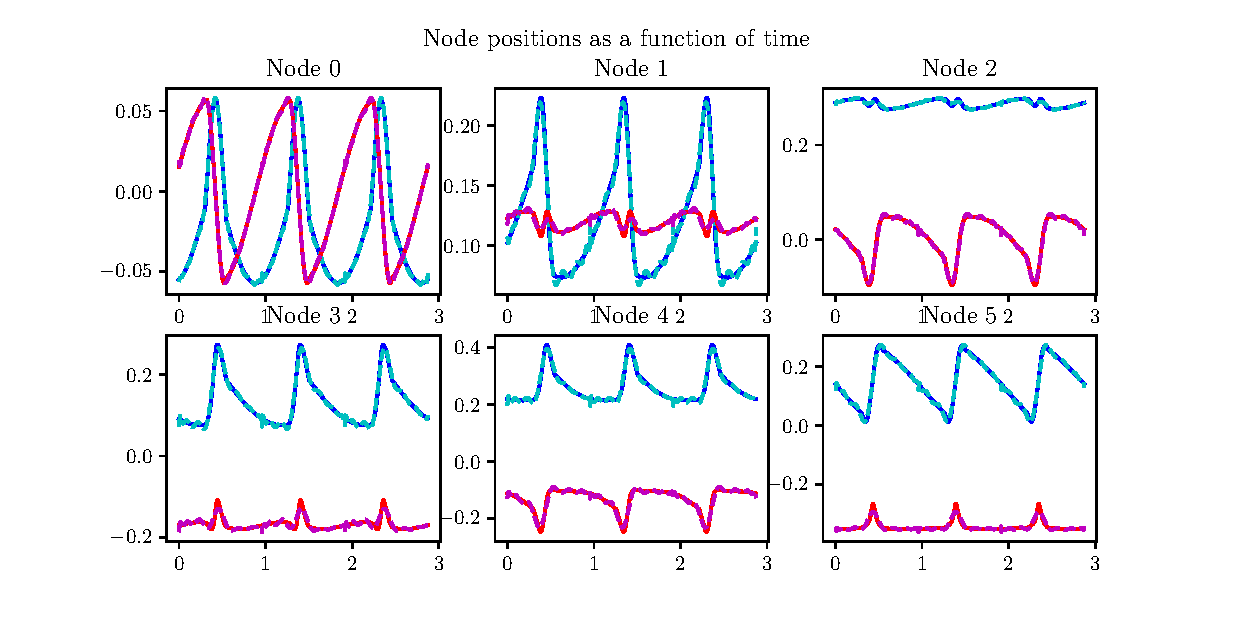
\includegraphics[width=\textwidth]{images/4/4_node-positions-fct-of-time.eps}
    \caption[Comparison between actual node trajectories and approximated trajectories over three leg cycles]{Comparison between actual node trajectories and approximated trajectories over three leg cycles. The original node position in $x$ is given in blue, the polynomial fit is given in cyan, the original node position in $y$ is given in red, and the polynomial fit is given in magenta}
    \label{fig:4_node-positions-fct-of-time}
\end{figure}

\subsubsection{Dynamic Model}

The dynamic model was fully developed using the same set equations as shown for the 3-DoF series-articulated topology. It was found, however, that this approach requires the use of Lagrange multipliers to represent the constraints applied to the leg \cite{nansai_dynamic_2013}. Without these, for a constant motor velocity during the contact and flight phases, the inertial terms are equal to zero. Equally, the external force is mostly lost. Both these significant inaccuracies are captured in Figure \ref{fig:4_jansen-torques}.

\begin{figure}
    \centering
    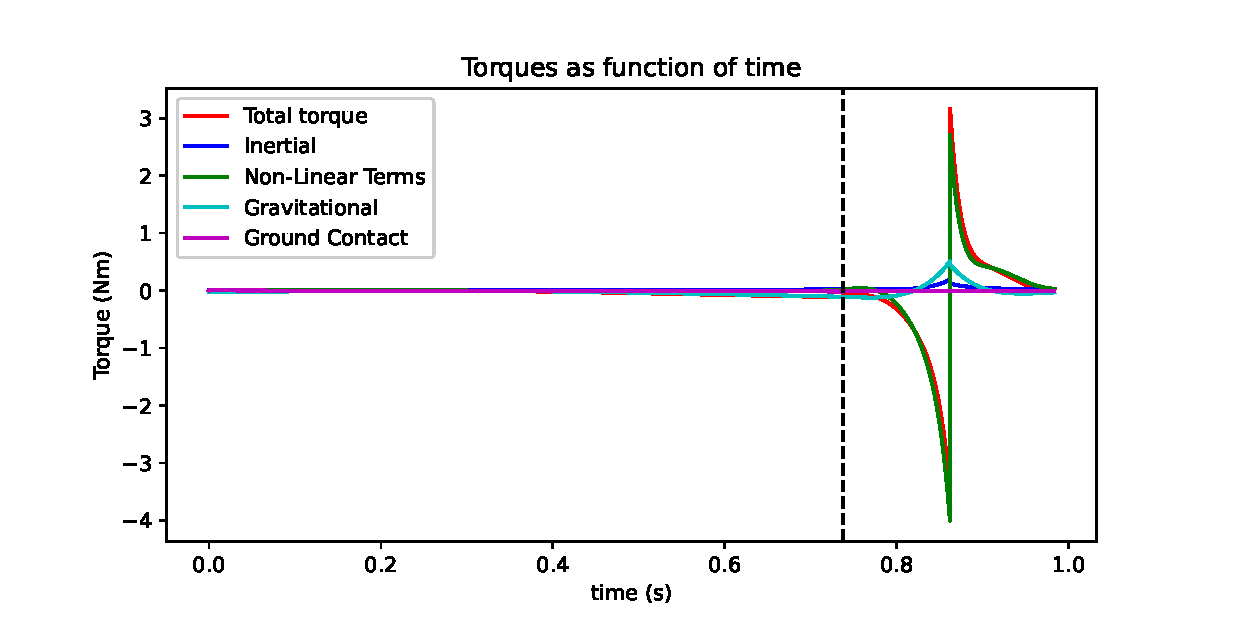
\includegraphics[width=\textwidth]{images/4/4_jansen-torques.eps}
    \caption[Improper Jansen torques found in dynamic model as a function of time over a leg cycle]{Improper Jansen torques found in dynamic model as a function of time over a leg cycle. The black dotted line indicates when the leg shifts from the ground contact phase (leg must carry weight of the robot) to flight phase.}
    \label{fig:4_jansen-torques}
\end{figure}

The leg dynamics were instead developed using Free Body Diagrams to determine the reaction forces at each link, beginning at the foot at Node-5 and working up to the actuator; a sample diagram is given by Figure \ref{fig:4_jansen-free-body-diagram}. The equations for each node are presented from (\ref{eq:jansen_reaction_5}) to (\ref{eq:jansen_reaction_torque}) in the order in which they are solved for; reaction $R_i$ correspond to the internal forces required to achieve the node accelerations $\ddot{x_i}$ and $\ddot{y_i}$. $\tau$ represents the output torque at the actuator, while mass $m_i$ represents the mass of link $i$ as per Figure \ref{fig:4_jansen-mechanism-patnaik}. Node-1 and Node-2 were not analysed directly; instead, links $\ell_2$, $\ell_{9}$ and $ell_{10}$ were treated as a solid body, and the sum of moments, illustrated in Figure \ref{fig:4_jansen_fbd_solid_body}, was solved for $R_1$.

\begin{figure}
    \centering
    \includegraphics[width=0.7\textwidth]{images/4/4_jansen_fbd_example.png}
    \caption{Sample Free-Body Diagram for Node-5}
    \label{fig:4_jansen-free-body-diagram}
\end{figure}

\begin{figure}
    \centering
    \includegraphics[width=0.8\textwidth]{images/4/4_jansen_fbd_solid_body.png}
    \caption{Free-Body Diagram for solid body composed of links $\ell_2$, $\ell_9$ and $\ell_{10}$}
    \label{fig:4_jansen_fbd_solid_body}
\end{figure}

\begin{align}
    R_5 &= \frac{(\frac{m_4+m_5}{2})(\ddot{y_5} + g - \ddot{x_5}\tan\theta_4) - F_e}{\sin\theta_5 - \cos\theta_5\tan\theta_4} \label{eq:jansen_reaction_5}
    \\
    R_4 &= \frac{(\frac{m_4+m_5}{2}) - R_5\cos\theta_5}{\cos\theta_4}
    \\
    R_7 &= \frac{(\frac{m_3+m_7}{2})(\ddot{y_4} + g - \ddot{x_4}\tan\theta_3) + R_4(\sin\theta_4 - \cos\theta_4\tan\theta_3)}{\sin\theta_7 - \cos\theta_7\tan\theta_3}
    \\
    R_3 &= \frac{(\frac{m_3+m_7}{2})\ddot{x_4} - R_7\cos\theta_7 + R_4\cos\theta_4}{\cos\theta_3}
    \\
    R_8 &= \frac{(\frac{m_6+m_8}{2})(\ddot{y_3} + g - \ddot{x_3}\tan\theta_3) + R_5(\sin\theta_5 - \cos\theta_5\tan\theta_6)}{\sin\theta_8 - \cos\theta_8\tan\theta_6} \\
    &\quad +  \frac{R_7(\sin\theta_6-\cos\theta_7\tan\theta_7)}{\sin\theta_8 - \cos\theta_8\tan\theta_6}
    \\
    R_6 &= \frac{(\frac{m_6+m_8}{2})\ddot{x_3} - R_8\cos\theta_8 + R_5\cos\theta_5 + R_7\cos\theta_7}{\cos\theta_6}
    \\
    \alpha &= \frac{\sqrt{\ddot{x}_2^2 + \ddot{y}_2^2} \cos\left(\theta_3 - \left(\frac{\pi}{2}+\theta_{10}\right)\right)}{\ell_{10}}
    \\
    R_1 &= \frac{\left(\frac{m_1+m_2+m_9}{2}\ell_9^2 + \frac{m_2+m_3+m_10}{2}\ell_{10}^2\right)\alpha + R_3 \ell_{10} \left(\cos\theta_3 \sin\theta_{10} + \sin\theta_3 \cos\theta{10} \right)}{\cos\theta_1 \sin\theta_9 + \sin\theta_1 \cos\theta_9}
    \\
	\tau &= \frac{m_0+m_1+m_6}{2} g \ell_0 \cos\theta_0 + R_1 \ell_0 (\sin\theta_1 \cos\theta_0 - \cos\theta_1 \sin\theta_0) \\
	&\quad + R_6 \ell_0 (\sin\theta_6 \cos\theta_0 - \cos\theta_6 \sin\theta_0) \label{eq:jansen_reaction_torque}
\end{align}

For the reaction $R_5$, the external force term $F_e$ represents the mass of the robot which must be held up by the leg, equal to the sum of all link masses and one third the torso mass of the robot, as the torso mass is shared between the three legs participating in the stable stance at any time. $F_e$ is therefore only present in the equation during the stance phase, when the leg is in contact with the ground. The link masses are split between their extremities and link inertias are neglected.

\subsubsection{Singularities}

Previously, a free body diagram was developed for each node, and link reaction equations derived. This methodology resulted in three additional equations.

\begin{align}
    R_2 &= \frac{(m_2+m_{10})\ddot{x_2} - R_{10}\cos\theta_{10} + R_3\cos\theta_3}{\cos\theta_2}
    \\
    R_9 &= \frac{(m_1+m_9)(\ddot{y_1} + g - \ddot{x_1}\tan\theta_1) + R_2(\sin\theta_2 - \cos\theta_2 \tan\theta_1)}{\sin\theta_9 - \cos\theta_9 \tan\theta_1}
    \\
    R_{10} &= \frac{(m_2+m_10)(\ddot{y_2} + g - \ddot{x_2}\tan\theta_2) + R_3(\sin\theta_3 - \cos\theta_3 \tan\theta_2)}{\sin\theta_{10} - \cos\theta_{10} \tan\theta_2} \label{eq:jansen_R10}
\end{align}

Using this method gave the torque graph shown in Figure \ref{fig:5_jansen_torque_invalid}. The massive torque spikes can be traced back to the reaction force $R_{10}$, shown in Figure \ref{fig:5_jansen_R10}.

\begin{figure}[b]
    \centering
    \includegraphics[width=\textwidth]{images/5/5_torque_invalid.png}
    \caption{Torque output of Jansen linkage over a three leg cycles without correcting for singularities}
    \label{fig:5_jansen_torque_invalid}
\end{figure}

\begin{figure}
    \centering
    \includegraphics[width=\textwidth]{images/5/5_R10.png}
    \caption{Reaction $R_{10}$ as a function of time}
    \label{fig:5_jansen_R10}
\end{figure}

These spikes are largely explained by the presence of modelling singularities; positions in which the reaction expressions tend towards infinity due to the presence of an asymptotic function. The force spikes present in Figure \ref{fig:5_jansen_R10} align chronologically with the times during which $R_{10}$'s denominator as defined in (\ref{eq:jansen_R10}) is equal to zero, and thus there is a reaction of infinite amplitude. Since reaction $R_{10}$ is used to determine the reactions $R_1$, $R_2$ and $R_9$, and subsequently the actuator torque $\tau$, these all exhibit the same large spikes, as shown in Figure \ref{fig:5_jansen_reactions_invalid}.

\begin{figure}
    \centering
    \includegraphics[width=\textwidth]{images/5/5_R10_denominator.png}
    \caption[Factors of $R_{10}$ denominator]{Factors of $R_{10}$ denominator. As per (\ref{eq:jansen_R10}), the denominator takes the form $\sin\theta_{10} - \cos\theta_{10}\tan\theta_2$}
    \label{fig:5_jansen_R10_denom}
\end{figure}

\begin{figure}
    \centering
    \includegraphics[width=\textwidth]{images/5/5_reactions_over_time_invalid.png}
    \caption[Reaction forces of Jansen linkage over a three leg cycles without correcting for singularities]{Reaction forces of Jansen linkage over a three leg cycles without correcting for singularities. Reaction $R_{10}$ is not shown, but exhibits a similar form to reactions 1, 2 and 9}
    \label{fig:5_jansen_reactions_invalid}
\end{figure}

It is worth noting that this singularity is not mechanical; one of the singular leg configurations is shown in Figure \ref{fig:5_jansen_singular_configuration_1}. The leg is fully capable of moving in and out of this position. The singularity is thus a consequence of the modelling technique, and not the leg design.

\begin{figure}
    \centering
    \includegraphics[width=0.8\textwidth]{images/5/5_R10_overflow_singular_configuration_1.png}
    \caption[Jansen linkage leg configuration during larger of the two singularities]{Jansen linkage leg configuration during larger of the two singularities. The left red dot represents the actuator, the right one represents the pin, the red link represents link $R_{10}$, for whom the reaction force tends towards infinity, and the blue curve represents the trajectory taken by the foot}
    \label{fig:5_jansen_singular_configuration_1}
\end{figure}

When the Jacobian is used for forward and inverse kinematics, and the dynamic model, techniques such the damped least-squares method or Moore-Penrose Pseudoinverse are used to approximate the appropriate value when such as singularity is found \cite{chiaverini_review_1994}\cite{sciencedirect_moore-penrose_nodate}. Alternatively, treating links $\ell_2$, $\ell_9$ and $\ell_{10}$ as forming a solid body avoids the mathematically singular configurations present in (\ref{eq:jansen_R10}).

\begin{comment}
%%%%%%%%%%%%%%%%%%%%%%%%%%%%%%%%%%%%%%%%%%%%%%%%%%%%%%%%%%%
%  3-DoF series-articulated
%%%%%%%%%%%%%%%%%%%%%%%%%%%%%%%%%%%%%%%%%%%%%%%%%%%%%%%%%%%
\subsection{Underactuated Spatial Mechanism}

Whereas the proportions of other leg topologies are based on existing quadrupeds, the underactuated configuration with three sets of linkages must undergo more careful deliberation, as this design will result in an uncontrolled degree of freedom whose orientation should be placed to maximize performance. Sample configurations are shown in Figure \ref{fig:parallel_concept_top}.

\begin{figure}
    \centering
    \includegraphics[width=0.8\textwidth]{4/4_parallel_top.png}
    \caption{Possible configurations for underactuated spatial leg topology}
    \label{fig:parallel_concept_top}
\end{figure}
\end{comment}
\section{Simulation} \label{sec:simulation}

%%%%%%%%%%%%%%%%%%%%%%%%%%%%%%%%%%%%%%%%%%%%%%%%%%%%%%%%%%%
%  Standard Measurements
%%%%%%%%%%%%%%%%%%%%%%%%%%%%%%%%%%%%%%%%%%%%%%%%%%%%%%%%%%%
\subsection{Standard Measurements}

In order to provide a relatively fair comparison between leg topologies, all designs share the same robot mass, torso height, walking speed, and link densities. ANYmal was used as a reference for all but the last of these values \cite{hutter_anymal_2016}. All robots have a torso mass of 30kg and a torso height of 0.35m. The torso height was found by taking the link lengths of ANYmal and finding the torso height for a configuration where the upper and lower links are separated by $90^{\circ}$ and the foot is found under the hip flexion/extension actuator, as shown in Figure \ref{fig:torso_height}. The robots move at a walking speed of $0.3\frac{m}{s}$, which is equal to the static walking speed of ANYmal. Links are composed of tubes of aluminium 6061 with a density of $2700\frac{kg}{m^3}$, with outer diameter $d_o=0.0440m$ and inner diameter $d_i=0.0408m$. Finally, the robots use HEBI Robotics X8-16 actuators as a stand-in for ANYdrives with peak torques of $38Nm$ and masses of $0.49kg$ \cite{hebi_robotics_x-series_nodate}.

\begin{figure}[b]
    \centering
    \includegraphics[width=0.5\textwidth]{5/5_torso_height.png}
    \caption{Simple calculation to determine reference robot torso height}
    \label{fig:torso_height}
\end{figure}

While Cost of Transportation tends to be inversely proportionate to the velocity of the robot, safe operation around humans is a higher priority than energy efficiency for the application defined in Section \ref{sec:app-metrics}, and thus a static walking gait was selected instead of trotting or bounding \cite{bledt_mit_2018}\cite{hutter_toward_2014}. The simple static walking gait developed by Hutter et al. was selected for this thesis as it is statically stable and simple to implement \cite{hutter_toward_2014}.

In order to simplify the analysis, each topology is treated as a robotic arm, where the foot is considered as the robot end-effector. The ground contact forces resulting from the robot weight are then represented as a load applied to the end-effector. To simulate these configurations, the robot body is considered fixed to the inertial reference frame and the robot foot is constrained to move in a deterministic trajectory selected to maintain the constant torso velocity of $0.3\frac{m}{s}$. This is synonymous to a person running on a treadmill.

%%%%%%%%%%%%%%%%%%%%%%%%%%%%%%%%%%%%%%%%%%%%%%%%%%%%%%%%%%%
%  Jansen linkage simulation procedure
%%%%%%%%%%%%%%%%%%%%%%%%%%%%%%%%%%%%%%%%%%%%%%%%%%%%%%%%%%%
\subsection{Jansen Linkage Simulation Procedure}

First, the Jansen linkage based leg topology was run through a full cycle, from $\theta_0=0^{\circ}$ to $\theta_0=360^{\circ}$. The points at which the foot makes contact with the ground $x_{contact}$ at $\theta_{0_{contact}}$ and lifts off the ground $x_{liftoff}$ at $\theta_{0_{liftoff}}$ were recorded. The total stride length $d_s$ is given by

\begin{equation}
    d_s = x_{contact} - x_{liftoff}
\end{equation}

Each leg is in contact with the ground for three quarters of the total leg cycle \cite{hutter_toward_2014}. Therefore the total distance traversed per cycle is given by

\begin{equation}
    d_c = d_s \times \frac{4}{3}
\end{equation}

Since the robots walk at a speed of $0.3\frac{m}{s}$, the time to complete a cycle is given by

\begin{equation}
    t_c = \frac{d_c}{0.3}
\end{equation}

where three quarters of the time is spent in the contact phase (foot in contact with the ground) and a quarter is spent in the flight phase (foot not in contact with the ground).

The simulation was run in the following manner. For a certain number of time steps of size $t_{step}$ between $t = 0$ and $t = t_c$:

\begin{enumerate}
    \item Calculate the current actuator angle for time step $k$ as $\theta_{0_k} = \theta_{0_{k-1}} + \dot{\theta}_{gf} t_{step}$, where $\dot{\theta}_{gf}$ is either $\dot{\theta}_{0_{stance}}$ or $\dot{\theta}_{0_{flight}}$, depending on whether the leg is in stance or flight phase
    \item Using the four bar linkage equations from (\ref{eq:4-four-bar-linkage-first}) to (\ref{eq:4-four-bar-linkage-last}), find the position of each node along the base $x$ and $y$. The foot positions $x_5$ and $y_5$ were also used for the 2-DoF series-articulated leg topology
    \item Create a polynomial fit for the position of each node with respect to time using the simulation data \cite{harris_array_2020}
    \item Derive the polynomial node positions with respect to time twice in order to obtain the expression of each node acceleration in $x$ and $y$ with respect to time.
    \item Calculate the actuator torque at each time step as expressed by (\ref{eq:jansen_reaction_torque}) using the reaction equations expressed by (\ref{eq:jansen_reaction_5}) through (\ref{eq:jansen_reaction_torque})
\end{enumerate}

Step 4 was done to avoid small denominator division; while the node velocities and accelerations could be calculated using

\begin{align} \label{eq:small_denom}
    \dot{x}_k &= \frac{x_k - x_{k-1}}{t_{step}}
    \\
    \ddot{x}_k &= \frac{\dot{x}_k - \dot{x}_{k-1}}{t_{step}}
\end{align}

, a small time step results in accelerations on the order of $10^6 \frac{m}{s}$, whereas deriving a symbolic representation of the node positions results in realistic values.

\subsubsection{Polynomial Fit}

\begin{figure}
    \centering
    \includegraphics[width=\textwidth]{images/5/x5_jump.png}
    \caption[Instantaneous position change due to polynomial fit being applied at a per-cycle level.]{Instantaneous position change due to polynomial fit being applied at a per-cycle level. The black line indicates the transition from one leg cycle to the next and coincides with the spike, further amplified after deriving for the node velocity and acceleration}
    \label{fig:5_x5_jump}
\end{figure}

In both Figures \ref{fig:5_comparison_torques} and \ref{fig:5_comparison_work} of the comparison, the Jansen mechanism exhibits large spikes. These are due to the manner in which the node accelerations are determined; the polynomial function used to approximate each position was fit to a single leg cycle; between cycles, there is an near-instantaneous jump between of node position due to the approximations not beginning and ending at the same position, demonstrated in Figure \ref{fig:5_x5_jump}. When derived to obtain the node velocity and acceleration, this instantaneous jump is amplified, resulting in the large spikes. As these spikes are virtually instantaneous, however, they perform limited damage when measuring power consumption. Additionally, the actual position curve as shown in Figure \ref{fig:5_x5_jump} is smooth, and thus the true acceleration would be near zero and the leg would not experience a torque spike.

%%%%%%%%%%%%%%%%%%%%%%%%%%%%%%%%%%%%%%%%%%%%%%%%%%%%%%%%%%%
%  2-dof series-articulated simulation procedure
%%%%%%%%%%%%%%%%%%%%%%%%%%%%%%%%%%%%%%%%%%%%%%%%%%%%%%%%%%%
\subsection{2-DoF Series-Articulated Simulation Procedure}

First, the foot position data and time step data calculated by the Jansen linkage were imported. The simulation was performed in two passes. The first uses the inverse kinematic equations to calculate the joint positions $\theta_1$ and $\theta_2$ at each time step. In order to avoid small denominator division as per (\ref{eq:small_denom}), a polynomial approximation for the joint angles $\theta_1$ and $\theta_2$ was developed and derived twice to obtain the angular velocities and angular accelerations. The second pass calculates the joint torques $\tau_1$ and $\tau_2$ at each time step using the dynamic equation from (\ref{eq:euler-lagrange}).

\subsubsection{Polynomial Fit}

The order of the polynomial approximation influences how well the equation fits the data, in this case joint position $\theta_1$ and $\theta_2$. A higher order polynomial approximation will fit the data better, as shown in Figure \ref{fig:5_2dof_angles_approx_7_15}, but will result in larger perturbations in derivative expressions, as shown in Figure \ref{fig:5_2dof_torques_approx_7_15}. A lower order polynomial will not fit the data as well, but will provide smoother derivative expressions. A polynomial approximation of 9th degree was chosen, as it was the highest order which did not experience large perturbations and exceed the $38Nm$ limit. The resulting joint torques are shown in the comparison section.

\begin{figure}
    \centering
    \includegraphics[width=\textwidth]{images/5/2dof_angles_poly7poly15.png}
    \caption{2-DoF series-articulated joint angles and polynomial approximations for 7th and 15th degree}
    \label{fig:5_2dof_angles_approx_7_15}
\end{figure}

\begin{figure}
    \centering
    \includegraphics[width=\textwidth]{images/5/2dof_torques_poly7poly15.png}
    \caption{2-DoF series-articulated joint torques for polynomial approximation of 7th and 15th degree}
    \label{fig:5_2dof_torques_approx_7_15}
\end{figure}

%%%%%%%%%%%%%%%%%%%%%%%%%%%%%%%%%%%%%%%%%%%%%%%%%%%%%%%%%%%
%  Comparison
%%%%%%%%%%%%%%%%%%%%%%%%%%%%%%%%%%%%%%%%%%%%%%%%%%%%%%%%%%%
\subsection{Comparison}

Joint torques are given in figure \ref{fig:5_comparison_torques}.

\begin{figure}
    \centering
    \includegraphics[width=\textwidth]{images/5/5_comparison_torques.png}
    \caption{Torques generated by each joint on Jansen linkage and 2-DoF series-articulated leg topologies}
    \label{fig:5_comparison_torques}
\end{figure}

The mechanical work performed during step $k$ is equal to the dot product of the joint torques and joint displacements; the performed work is shown in Figure \ref{fig:5_comparison_work}.

\begin{equation}
W_k = \tau_k \cdot (\theta_{k} - \theta_{k-1})
\end{equation}

\begin{figure}
    \centering
    \includegraphics[width=\textwidth]{images/5/5_comparison_work.png}
    \caption{Work performed by each joint on Jansen linkage and 2-DoF series-articulated leg topologies}
    \label{fig:5_comparison_work}
\end{figure}

The average mechanical power expended is calculated as

\begin{equation}
    P_{mechanical} = \frac{\sum_{k=0}^n W_k}{t_{total}}
\end{equation}

where the work is summed over all $n$ time steps of the simulation and divided by the total simulation time $t_{total}$.

As described above, the Jansen linkage leg topology exhibits large torque spikes when the leg transitions from one leg cycle to the next as there is an instantaneous position jump. While the true torque during these spikes could be approximated as the torques before and after the spike, a more conservative approach is taken. From Patnaik's work, it can be noted that the largest experienced torque is less than two times the size of the second largest during a leg cycle. Double the largest torque, excluding the instantaneous peaks, was therefore selected for the calculation of $\phi$.

The proprioceptive force sensitivity $\Pi$ as defined by (\ref{eq:proprioceptive-force-sensitivity}) only considers the leg Jacobian and external force $F$. This is equivalent to a static configuration with no gravity; for the Jansen linkage, all joint accelerations are set to zero. For the 2-DoF series-articulated leg the inertia, non-linear and gravitational terms are set to zero. The ground contact force is set to $140N$ for both leg topologies as it is the maximum external force experienced by the Jansen mechanism, and the force variation $\epsilon$ is set to $1N$. Both legs use the same foot position for the calculation of $\Pi$, as the proprioceptive force sensitivyt varies with respect to the Jacobian and thus the foot position. As the Jansen linkage was not modelled using the Jacobian method, Equations (\ref{eq:jansen_reaction_5}) through (\ref{eq:jansen_reaction_torque}) were used to determine $\Pi$.

\begin{table}[h]
    \centering
    \begin{tabular}{lcc}
        \textbf{Metric} & \textbf{Jansen} & \textbf{2-DoF} \\
        \hline
        Power Consumption (W) & $4.2$ & $15.5$ \\
        $\phi$ (Nm) & $9.0$ & $51.0$ \\
        $\Pi$ (Nm) & $0.0185$ & $0.1929$
    \end{tabular}
    \caption{Performance metric results for Jansen linkage and 2-DoF series-articulated based leg topologies}
    \label{tab:results}
\end{table}


\section{Discussion}

The Jansen linkage was first used by Theo Jansen in the Strandbeest, a mobile art piece that could traverse the environment using nothing more than wind power \cite{jansen_strandbeest_nodate}. The philosophy of efficiency is certainly confirmed in the simulation results. The Jansen linkage leg topology expends approximately a third the energy of the 2-DoF series-articulated leg topology, with $4.2W$ and $15.5W$ average power consumption respectively. This is explained both by having an smaller average actuator torque, as well as using a single actuator instead of two. Having less actuators, as well as a lower required torque, are equally beneficial when comparing the leg topologies' values of $\phi$; $\phi_{jansen}$ is under a fifth the value of $\phi_{2-DoF}$. The total cost of actuators to power the Jansen linkage would thus be significantly lower than the cost to actuate the 2-DoF series-articulated leg.

Where the Jansen mechanism leads in power consumption and actuator cost, it falls behind in workspace volume, force envelope volume and proprioceptive force sensitivity. Both workspace volume $V$ and force envelope volume $\Psi$ were not measured numerically as the result can be determined heuristically; the Jansen linkage is constrained to a predetermined foot trajectory and as such, has a vastly inferior workspace and by extension force envelope volume. It is worth noting that, while volume is a three-dimensional measure, leg movement was constrained during simulations to the sagittal plane, and the hip adduction/abduction is assumed to be controlled by other means, such as the implementations presented in Appendix \ref{app:A}; both leg's out of sagittal plane mobility are assumed to be equal. The Jansen linkage also demonstrates worse proprioceptive force sensitivity $\Pi$ than the 2-DoF series-articulated leg topology, with $0.0185Nm$ and $0.1929Nm$ respectively. This may be explained by antagonistic forces consuming some of the input force \cite{hubicki_atrias_2016}. The magnitude of the difference is dubious, however, as Kalouche found a proprioceptive force sensitivity for a 2-DoF series-articulated leg topology of $0.0667Nm$ \cite{kalouche_design_2016}. Either value remains higher than that of the Jansen linkage.

From Section \ref{sec:app-metrics}, it was determined that the robot should be able to navigate mildly unstructured but not overly hostile terrain. It should be able to turn and move at a maximum velocity that is safe for operation near humans, and operate for a reasonable period of time on battery or solar power. These design criteria suggest, in tandem, an emphasis on energy efficiency with only mild requirements in terms of mobility. Further, while proprioceptive force sensitivity is essential to permit accurate force control, external sensors can be used to measure foot contact forces, wind forces, etc. at the cost of additional design complexity. While the 2-DoF series-articulated leg topology has far superior leg mobility, measured by force envelope volume and workspace volume, the selected working environment is only mildly unstructured, and thus the additional mobility is of limited benefit. In contrast, the 2-DoF series-articulated topology has significantly higher power consumption. The Jansen linkage is therefore the preferred option for a robot performing litter collection in a beachfront environment.

\subsection{Limitations}

The modelling and simulation of both leg topologies suffered from various methodological limitations. A flagrant example is the chosen foot trajectory; while the Jansen linkage is constrained to a single foot trajectory, the 2-DoF series-articulated leg topology has a significantly larger work-space to play in, and therefore there may be a more efficient trajectory to follow than that of the Jansen linkage. For example, a foot trajectory which barely rises off the ground is likely more efficient than that of the Jansen linkage, which rises quite significantly in the $y$ direction.

The knee actuator for the 2-DoF series-articulated leg is aligned coaxially with the hip actuator in accordance with most series-articulated legged robots \cite{bledt_mit_2018}\cite{katz_mini_2019}\cite{grimminger_open_2020}. This approach requires the use of a pulley or linkage to manipulate the knee remotely. The energy which would be lost in this transfer mechanism is not considered when calculating the proprioceptive force transparency. Equally, the mass of the transfer mechanism is not considered, although this is likely of insignificant amplitude when compared to the torso and leg masses.

The use of polynomial functions to approximate the node positions for the Jansen linkage and actuator positions for the 2-DoF series-articulated leg introduced inaccuracies. Figures \ref{fig:5_2dof_angles_approx_7_15} and \ref{fig:5_2dof_torques_approx_7_15} demonstrate how the degree of the polynomial function influences both the accuracy of the initial fit, as well as the oscillatory behavior that appears when the fit is derived. Additionally, Figure \ref{fig:5_x5_jump} demonstrates how applying the polynomial approximation to a single cycle can introduce instantaneous position jumps which propagate into accelerations and finally actuator torques. These were a consequence of modelling backwards; the simulation procedure began with the desired position of each node or actuator angle at each time step and ended with the actuator torques, instead of applying actuator torques and calculating the resulting node or actuator angle. Since this approach does account for real actuator acceleration and torque limits, the rise time is effectively zero between the current state and the next, and thus joint and node accelerations explode. Properly modelling both legs using a controller with rate limiters on joint accelerations and torques would resolve these irregularities.

Within the selected simulation procedure, two major errors occured. First, the non-linear terms $C(q,\dot{q})$ in the 2-DoF series-articulate model are always zero; the equations were likely miscalculated. The torso velocity was set to $0.3\frac{m}{s}$; from this, the required velocity of the foot while on the ground was determined. Tn the simulation for the Jansen linkage, however, the angular velocity during the ground contact phase was set as constant instead of the foot velocity. While this would result in the same torso velocity as it is akin to using the average angular velocity at all times, the foot ground velocity should be not constant. If simulated correctly, the angular velocity would vary, and thus the results may have varied.

\subsection{Conclusion}

The performance metrics presented in this thesis cover the diverse goals of legged robots, from explosive and dynamic quadrupeds, to simple and cost effective ones. A subset of these metrics were selected to evaluate two leg topologies for a beachfront litter collection application; a Jansen linkage based leg and a 2-DoF series-articulated leg. The Jansen linkage was successfully determined to be the optimal leg design for this application, with some caveats in the modelling and simulation of the topologies. Future work correcting these shortcomings would further validate the choice of leg topology for the given use-case and performance metrics. Additionally, analyzing the other leg topology archetypes presented would either reinforce the selected leg topology or determine a superior one.
\newpage

\bibliographystyle{IEEEtran}
\bibliography{references.bib}

\newpage

\fancyhead[R]{A}

\appendix
\section{Enabling Hip Abduction} \label{app:A}

Below are figures of how planar leg topologies (those whose movement is constrainted to the sagittal plane) can enable turning.

\begin{figure}[h]
    \centering
    \includegraphics[width=\textwidth]{4/4_serial.png}
    \caption[Series-articulated full body configurations]{Approaches to modifying the classic 3-DoF serial-actuated topology for an under-actuated quadruped. From left to right: 2 sagittal plane actuators with rear leg steering, 2 sagittal plane actuators with rear and front leg steering, 1 sagittal and 1 frontal actuator with spring for 3rd DoF}
    \label{fig:serial_concepts}
\end{figure}

\begin{figure}[h]
    \centering
    \includegraphics[width=\textwidth]{4/4_parallel.png}
    \caption[Parallel-articulated full body configurations]{Approaches to modifying the 2-DoF parallel topology found in Stanford Doggo and Minitaur for an under-actuated quadruped. From left to right: 2 sagittal plane actuators with rear leg steering, 2 sagittal plane actuators with rear and front leg steering, 1 sagittal and 1 frontal actuator with spring for 3rd DoF}
    \label{fig:parallel_concepts}
\end{figure}

\begin{figure}[h]
    \centering
    \includegraphics[width=\textwidth]{4/4_triple_parallel.png}
    \caption[Underactuated spatial full body configurations]{Approaches to modifying the 3-DoF parallel-articulated topology for an under-actuated quadruped. Left model uses a spring in place of a third actuator at the hip. Right model uses a spring at the knee joint}
    \label{fig:triple_parallel_concepts}
\end{figure}

\end{document}
